
\documentclass{article} % For LaTeX2e
\usepackage{iclr2026_conference,times}

% Optional math commands from https://github.com/goodfeli/dlbook_notation.
\input{math_commands.tex}

\usepackage{hyperref}
\usepackage{url}

\usepackage{natbib}
\usepackage{algorithm}
\usepackage{algorithmic}

% Mathematical packages
\usepackage{amsmath}
\usepackage{amssymb}
\usepackage{amsthm}
\usepackage{mathtools}
\newtheorem{definition}{Definition}[section]

\usepackage{amsthm}
\usepackage{enumitem}
\usepackage{tikz}
\usepackage{multirow}
\usepackage{caption}
\usepackage{subcaption}
\usepackage{booktabs}




\title{Markovian Transformers for Informative Language Modeling}

% Authors must not appear in the submitted version. They should be hidden
% as long as the \iclrfinalcopy macro remains commented out below.
% Non-anonymous submissions will be rejected without review.

\author{Antiquus S.~Hippocampus, Natalia Cerebro \& Amelie P. Amygdale \thanks{ Use footnote for providing further information
about author (webpage, alternative address)---\emph{not} for acknowledging
funding agencies.  Funding acknowledgements go at the end of the paper.} \\
Department of Computer Science\\
Cranberry-Lemon University\\
Pittsburgh, PA 15213, USA \\
\texttt{\{hippo,brain,jen\}@cs.cranberry-lemon.edu} \\
\And
Ji Q. Ren \& Yevgeny LeNet \\
Department of Computational Neuroscience \\
University of the Witwatersrand \\
Joburg, South Africa \\
\texttt{\{robot,net\}@wits.ac.za} \\
\AND
Coauthor \\
Affiliation \\
Address \\
\texttt{email}
}

% The \author macro works with any number of authors. There are two commands
% used to separate the names and addresses of multiple authors: \And and \AND.
%
% Using \And between authors leaves it to \LaTeX{} to determine where to break
% the lines. Using \AND forces a linebreak at that point. So, if \LaTeX{}
% puts 3 of 4 authors names on the first line, and the last on the second
% line, try using \AND instead of \And before the third author name.

\newcommand{\fix}{\marginpar{FIX}}
\newcommand{\new}{\marginpar{NEW}}

%\iclrfinalcopy % Uncomment for camera-ready version, but NOT for submission.
\begin{document}


\maketitle

\begin{abstract}
Chain-of-Thought (CoT) reasoning often fails to faithfully reflect a language model's underlying decision process. We address this by introducing a \emph{Markovian} language model framework that can be understood as a reasoning autoencoder: it creates a text-based bottleneck where CoT serves as an intermediate representation, forcing the model to compress essential reasoning into interpretable text before making predictions. We train this system using a policy gradient algorithm inspired by Group Relative Policy Optimization (GRPO), with parallel sampling and actor reward gradients derived from the constraint that our reward model uses the same parameters $\theta$ as the policy model. This approach achieves a 33.2\% absolute accuracy improvement on GSM8K with Llama 3.1 8B. Comprehensive perturbation analysis across 29,440 comparison points and four model pairs demonstrates that Markovian training produces systematically higher sensitivity to CoT perturbations (effect differences +0.0154 to +0.3276), with 52.9\%--87.6\% consistency in showing greater fragility compared to Non-Markovian approaches. Cross-model evaluation confirms that learned CoTs generalize across architectures, indicating they capture transferable reasoning patterns rather than model-specific artifacts.
\end{abstract}

\section{Introduction}
\label{sec:intro}
The rapid advancement of language models (LMs) has led to impressive performance on complex cognitive tasks~\citep{NEURIPS2020_1457c0d6}. Yet it is often unclear \emph{why} an LM arrives at a particular conclusion~\citep{lamparth2023analyzing,burns2024discovering,gurnee2024language}, causing issues in high-stakes applications~\citep{Grabb2024.04.07.24305462,lamparth2024human,rivera2024escalation}. Traditional interpretability methods analyze hidden activations or attention patterns to extract ``explanations''~\citep{geiger2022inducing,geva2022transformer,meng2022locating,raukur2022toward,wang2022interpretability,lamparth2023analyzing,nanda2023progress}. Modern LMs, however, already generate coherent text: we might hope \emph{prompting} the model to articulate its reasoning (``Chain-of-Thought'' or CoT)~\citep{nye2022show,wei2022chain} would yield a faithful record of its thought process. 

Unfortunately, CoT explanations can be \emph{unfaithful}. For example, \citet{turpin2023language} show that spurious in-context biases often remain hidden in the CoT, and \citet{lanham2023measuring} find that altering CoT text may not affect the final answer. Such observations indicate that standard CoTs are not ``load-bearing.''

In this work, we take a \emph{pragmatic} approach to interpretability, focusing on \emph{informativeness} over full faithfulness. Rather than insisting the CoT mirrors the model's entire internal process, we require that \emph{the CoT alone suffices to produce the final answer}. In other words, if we remove the original prompt and rely only on the CoT, the model should still reach the correct output. This makes the CoT \emph{causally essential} and \emph{fragile}: changing it necessarily alters the prediction.

What distinguishes our approach is the clear distinction between the model \emph{relying on its CoT} versus generating \emph{more informative CoTs}. While traditional approaches train models to generate better-quality CoTs, they don't fundamentally change how the model uses them. Our Markovian framework, by contrast, forces the model to process information through the CoT bottleneck, making the CoT not just informative but \emph{causally load-bearing} for prediction.

For instance, Llama's CoT on arithmetic tasks changed dramatically after training. \textbf{Before training}, it simply listed all numbers and their (incorrect) sum (e.g., ``Sum = 76 + 90 + 92 + ... = 2314''). \textbf{After training}, it performed correct step-by-step calculations (e.g., ``calculate 6 + 89 = 95; Next, calculate 95 + 38 = 133...''), breaking the task into manageable steps that can be verified independently and enabling accurate answer prediction even when the original question is removed.

\paragraph{Recipient-Specific Compression.}
A key insight is that an \emph{informative} CoT can also serve as a \emph{recipient-specific compression} of the model's hidden knowledge: it distills the essential reasoning into text that another recipient (e.g.\ a different model or a human) can use to predict the same outcome. Our experiments confirm that the learned CoTs generalize across interpreters, suggesting that these textual explanations genuinely encode transferable problem-solving steps rather than model-specific quirks (Section~\ref{subsec:interp}).

\paragraph{Contributions.}
\begin{enumerate}
    \item We introduce a Markovian language model framework that structurally enforces Chain-of-Thought (CoT) generation to be causally essential, ensuring reliance on the CoT for predictions.
    \item We apply this framework to arithmetic problems (Mistral 7B) and the GSM8K dataset~\citep{cobbe2021gsm8k} (Llama 3.1 8B), observing a 33.2\% absolute improvement on GSM8K.
    \item We show through systematic perturbation analysis across four model pairs that Markovian training produces significantly higher sensitivity to CoT perturbations compared to Non-Markovian approaches, with effect differences ranging from +0.0154 to +0.3276 in log-probability sensitivity.
    \item We demonstrate cross-model transfer: CoTs trained on one model remain informative for other models. This underscores the CoT's \emph{recipient-specific} interpretability and suggests it captures a shared reasoning strategy.
\end{enumerate}

Section~\ref{sec:related_work} reviews related work, Section~\ref{sec:MLM} details our Markovian framework, and Section~\ref{sec:method} describes the RL training. Section~\ref{sec:experiments} presents empirical results, and Section~\ref{sec:disc} discusses limitations and future directions.


\begin{figure*}[t!]
  \centering
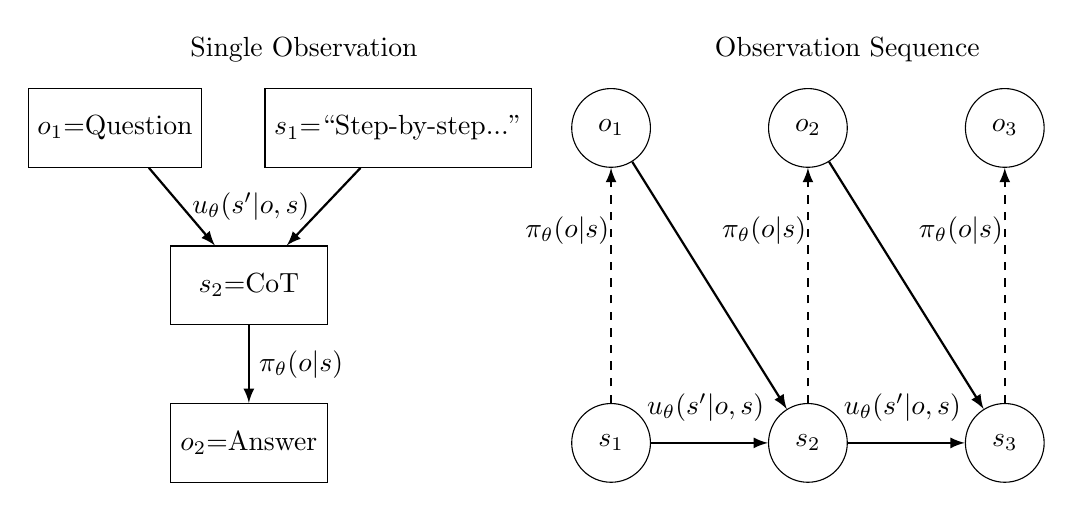
\begin{tikzpicture}[
    node distance=2cm,
    box/.style={rectangle, draw, minimum width=2cm, minimum height=1cm},
    circlebox/.style={circle, draw, minimum size=1cm},
    arrow/.style={->, thick},
    >=latex
]

% Left side: Single timestep
\node[box] (Q) at (-4.3,2) {$o_1$=Question};
\node[box] (S) at (-0.7,2) {$s_1$=``Step-by-step...''};
\node[box] (CoT) at (-2.6,0) {$s_2$=CoT};
\node[box] (A) at (-2.6,-2) {$o_2$=Answer};

\draw[arrow] (Q) -- node[right] {$u_\theta(s'|o,s)$} (CoT);
\draw[arrow] (S) -- (CoT);
\draw[arrow] (CoT) -- node[right] {$\pi_\theta(o|s)$} (A);

% Right side: Causal structure
% Observations
\node[circlebox] (o1) at (2,2) {$o_1$};
\node[circlebox] (o2) at (4.5,2) {$o_2$};
\node[circlebox] (o3) at (7,2) {$o_3$};

% States
\node[circlebox] (s1) at (2,-2) {$s_1$};
\node[circlebox] (s2) at (4.5,-2) {$s_2$};
\node[circlebox] (s3) at (7,-2) {$s_3$};

% Connections
\draw[arrow] (o1) to (s2);
\draw[arrow] (s1) to (s2);
\node[above] at (3.2,-1.85) {$u_\theta(s'|o,s)$};

\draw[arrow] (o2) to (s3);
\draw[arrow] (s2) to (s3);
\node[above] at (5.7,-1.85) {$u_\theta(s'|o,s)$};

% π(o|s) connections
\draw[arrow, dashed] (s1) to (o1);
\node[left] at (2.1,0.7) {$\pi_\theta(o|s)$};

\draw[arrow, dashed] (s2) to (o2);
\node[left] at (4.6,0.7) {$\pi_\theta(o|s)$};

\draw[arrow, dashed] (s3) to (o3);
\node[left] at (7.1,0.7) {$\pi_\theta(o|s)$};

% Labels
\node at (-1.9,3) {Single Observation};
\node at (5,3) {Observation Sequence};

\end{tikzpicture}
\caption{Markovian training as a reasoning autoencoder. Left: Single time-step process from Question to CoT to Answer, creating a text-based bottleneck where the CoT must capture all information needed for answer prediction. Right: Causal structure showing the generation of states from observations and previous states using the state update function $u_\theta(s'|o,s)$, and the prediction of observations from states using the policy $\pi_\theta(o|s)$. This architecture forces reasoning through an interpretable text bottleneck, but prevents direct backpropagation, necessitating RL-based gradient estimation.}
\label{fig:training-method-causal-final}
\end{figure*}

\begin{figure}[t]
  \centering
    \includegraphics[width=0.43\textwidth]{Figures/combined_normalized_reward_gp_smoothed.png}
    \caption{Normalized reward progression during Wikipedia continuation training across four model architectures. The normalized reward $\ln \pi_\theta(\text{ans} \mid \text{CoT}) - \ln \pi_\theta(\text{ans} \mid \text{CoT}')$ measures how much more informative the trained CoT becomes compared to baseline reasoning from the unmodified model. Each curve represents a different model architecture: Llama 3.1 8B (blue), Phi-3.5 Mini (orange), Qwen3 4B (green), and Mistral 7B (red). The plot uses Gaussian Process-style smoothing with confidence bands to highlight training trends. All models show consistent improvement in CoT informativeness, demonstrating the generalizability of the Markovian training approach across diverse architectures.}
    \label{fig:loss}
\end{figure}

\section{Related Work}
\label{sec:related_work}

Prior work shows that CoT prompting can boost performance on reasoning tasks \citep{wei2022chain, nye2022show}.
Whereas typical CoT prompting methods do not alter a pre-trained model's parameters, some prior approaches do fine-tune the model for CoT generation \citep{eric_star2022, zelikman2024quietstar, deepseekai2025}. Our work differs by removing the original question or passage from the answer-prediction context, which enforces a stronger causal reliance on the CoT.

Regarding faithfulness vs. interpretability, some authors discuss how a CoT may fail to reflect the true reason the LM arrived at its answer \citep{lanham2023measuring, turpin2023language}, since small changes in the CoT do not necessarily change the final prediction. \citet{zhou2023understanding} analyze CoT through an information-theoretic lens, finding that CoT can serve as a communication channel between different parts of a model. We build on these insights by \emph{training} the model to rely on this channel exclusively.

Architecturally, our Markovian LM shares structural similarities with state space models like RNNs \citep{rumelhart1986learning}, S4 \citep{gu2022efficientlymodelinglongsequences}, and Mamba \citep{gu2024mamba}, though with a key difference: MLMs have probabilistic state transitions to model token sampling, which necessitates gradient estimation methods such as policy gradient \citep{policy_gradient} rather than direct backpropagation. This probabilistic structure also resembles Kalman filters \citep{proto_pomdp1965}, Deep Variational Bayes Filters \citep{karl2017deepvariationalbayesfilters}, Deep Kalman Filters \citep{krishnan2015deepkalmanfilters}, and Variational Recurrent Neural Networks (VRNN) \citep{DBLP:journals/corr/ChungKDGCB15}, though we use categorical rather than Gaussian distributions for interpretable text generation. Other fine-tuned reasoning models mentioned above (R1, STaR, and QuietSTaR) have similar structure but allow seeing the full context before generating state/reasoning tokens, whereas our approach enforces a strict information bottleneck through the state.

\citet{lyu2023faithful} also consider restricting the model's ability to see the original input while generating the final answer. Their approach, however, involves rewriting the question in a structured formal language or code that is then executed. Our approach uses natural language for the reasoning state to preserve interpretability across diverse tasks.

\section{Markovian Language Models and Informativeness}
\label{sec:MLM}

Here we provide our formalism for Markovian Language Models (MLMs) and define \emph{informativeness}, which we use as a training objective within our novel structural framework.

\subsection{Markovian Language Models (MLM)}

A traditional LM can attend to the entire context when predicting the next token. This makes it possible for an LM to disregard the CoT or only partially rely on it. We impose a stricter, \emph{Markovian} structure\footnote{This structure can be viewed as a stochastic variant of a Moore machine where both the transition function ($u$) and output function ($\pi$) are probabilistic, and the input and output alphabets are identical ($O$). Alternatively, an MLM can be formalized as an F-coalgebra where F(S) = P(O) $\times$ P(S)$^O$, with P representing probability distributions.}:
\begin{definition}[Markovian LM]
A Markovian Language Model is a tuple $M=(\mathcal{O}, \mathcal{S}, \pi, u, s_1)$, where
\begin{itemize}
\item $\mathcal{O}$ is a set of observations (e.g., questions and answers in a QA task),
\item $\mathcal{S}$ is a set of states (e.g., CoT reasoning text),
\item $\pi: \mathcal{S}\rightarrow \Delta(\mathcal{O})$ is a policy that predicts the next observation from the state alone,
\item $u: \mathcal{O}\times\mathcal{S}\rightarrow \Delta(\mathcal{S})$ is a state update function (produces CoT from question and initial prompt),
\item $s_1\in \mathcal{S}$ is an initial state (starting CoT prompt).
\end{itemize}
\end{definition}

For example, in a math reasoning task, $o_1 \in \mathcal{O}$ might be a question, $s_1 \in \mathcal{S}$ is an initial CoT prompt like ``Let's solve this step-by-step:'', $s_2 \in \mathcal{S}$ is the generated reasoning chain, and $o_2 \in \mathcal{O}$ is the answer. The key idea is that $\pi$ can only see the CoT state $s_2$ when predicting $o_2$, forcing the CoT to contain all needed information. Intuitively, $\pi$ is the \emph{frozen} next-token predictor, and $u$ is the model's \emph{trainable} component that chooses how to produce the CoT from the latest observation and prior state. In our experiments, $\pi$ and $u$ share the same underlying transformer but we freeze the weights for $\pi$ while fine-tuning those used by $u$. 

\subsection{Data-Generating Distribution and Reward}

Let $P$ be the distribution over observations $x_1, x_2, \dots, x_T \in \mathcal{O}$. A trajectory $\tau$ is generated by:
\[
s_{t+1}\sim u(s_t, x_t), \quad x_{t+1}\sim P(x_{t+1}\mid x_{\le t}),
\]
with $s_1$ a fixed initial prompt. We define the \emph{reward} for a trajectory $\tau$ as:
\[
R_\theta(\tau)=\sum_{t=1}^T \left[\ln \pi_\theta(x_t\mid s_t)-\ln \pi_\theta(x_t\mid s'_t)\right],
\]
where $s'_t$ is generated by a \emph{baseline} update function $u'$, e.g., the \emph{untrained} model. In words, $R_\theta(\tau)$ measures how much more likely the correct observation $x_t$ is under the trained state $s_t$ compared to the baseline state $s'_t$.

\subsection{Informativeness Objective}

Conceptually, we aim to ensure that the CoT state serves as a critical bottleneck for information flow, making it causally essential for predictions. Formalizing this within our Markovian framework, we define:
\[
  J(\theta)=\mathbb{E}_{\tau \sim P,u_\theta,u'}\left[R_\theta(\tau)\right],
\]
where $\theta$ parameterizes $u_\theta$. Maximizing $J(\theta)$ ensures that the update function $u_\theta$ produces states $s_t$ that are \emph{informative} about future observations (relative to the baseline $u'$), thereby enforcing the CoT's role as a load-bearing component. We optimize $J(\theta)$ with policy gradient or PPO, sampling observations from $P$ and states from $u_\theta$ and $u'$.

\section{Methods}
\label{sec:method}

\subsection{Implementation as Question-Answer Pairs}
In many tasks like math problem solving, we have $T=2$ observations (question and answer) and implement the abstract MLM with a fixed maximum length for the CoT state. Let $\mathcal{V}$ be a token vocabulary. We set $\mathcal{O} = \mathcal{V}^N$ and $\mathcal{S} = \mathcal{V}^K$ for some $N, K \in \mathbb{N}$, where $K$ is the maximum tokens in the CoT. Note that while we limit the state to a maximum of $K$ tokens for implementation, we do not enforce fixed-length observations. 

Our conceptual arguments rely on $K < N$, as otherwise the model could simply write the predicted observation into the state. We satisfy this in our Wikipedia experiments (Sec~\ref{subsec:wikipedia}), and for other experiments we find empirically that the model does not learn this undesirable behavior due to the difficulty of predicting the answer directly without any CoT.

In this setting, we denote our states as $s_1 = \text{CoT}_{\text{init}}$ and $s_2 = \text{CoT}$, where $\text{CoT}_{\text{init}}$ is a task-specific prompt\footnote{The exact prompt template varies by task type, with each template specifying the task objective, allowed $\text{CoT}$ length, and an invitation to reason strategically. Full templates are provided in Sec~\ref{subsec:stability}.}. With pre-trained LM $\mathcal{L}$, we can implement our update function $u$ and policy $\pi$ using:
\[\ln u_\theta\!\bigl(s_2=\text{CoT}\mid q, s_1=\text{CoT}_{\text{init}}\bigr)
= \sum_{i=1}^{K} \ln \mathcal{L}_\theta\!\bigl(\text{concat}(q,\text{CoT}_{\text{init}},\text{CoT}_{<i})\bigr)[\text{CoT}_i], \]
\[\ln \pi_\theta(\text{ans}\mid \text{CoT})
= \sum_{i=1}^{N} \ln \mathcal{L}_\theta\!\bigl(\text{concat}(\text{CoT},\text{ans}_{<i})\bigr)[\text{ans}_i].\]

Crucially, we do \emph{not} allow the answer generation to attend back to the question $q$ directly; the question is replaced by the $\text{CoT}$. For each question $q$, we generate the baseline state $s'_2$ (which we denote as $\text{CoT}'$ in this setting) by prompting the unmodified pre-trained model with $q$ plus an initial instruction (e.g., 'Think step-by-step...'), and recording its raw output.

Our reward is:
$$
R_\theta = \ln \pi_\theta(\text{ans} \mid \text{CoT}) \;-\; \ln \pi_\theta(\text{ans} \mid \text{CoT}').
$$

\subsection{Policy Gradient with GRPO-Style Baseline}
\label{subsec:grpo}

Markovian training can be understood as training a \emph{reasoning autoencoder}, where the CoT serves as a text-based bottleneck between question and answer. Like traditional autoencoders, this architecture forces information compression, but the intermediate representation is interpretable text rather than latent vectors. This text bottleneck prevents direct backpropagation and necessitates reinforcement learning techniques for gradient estimation.

\subsubsection{Actor Reward Gradients: The Key Innovation}
Our approach differs fundamentally from standard reinforcement learning by using the \emph{same} transformer with weights $\theta$ as both the policy model and the reward model. This creates a crucial mathematical distinction from traditional policy gradient methods.

In classical policy gradient, the reward $R(\tau)$ is independent of the policy parameters, leading to the standard REINFORCE gradient:
$$\nabla_\theta \mathbb{E}_{\tau \sim P_\theta}[R(\tau)] = \mathbb{E}_{\tau \sim P_\theta}[R(\tau) \cdot \nabla_\theta \ln P_\theta(\tau)]$$

However, in our case, the reward is a function of the same parameters: $R_\theta(\tau) = \ln \pi_\theta(\text{ans} \mid \text{CoT})$. Applying the chain rule:
\[\nabla_\theta \,\mathbb{E}_{\tau \sim P_\theta}[R_\theta(\tau)]
= \mathbb{E}_{\tau \sim P_\theta}\!\big[R_\theta(\tau)\, \nabla_\theta \ln P_\theta(\tau) + \nabla_\theta R_\theta(\tau)\big].\]

This yields two terms: the standard policy gradient ($R_\theta(\tau) \cdot \nabla_\theta \ln P_\theta(\tau)$) and the direct reward gradient ($\nabla_\theta R_\theta(\tau)$). We include both terms with equal weight in our implementation.

\subsubsection{GRPO-Style Baseline with Local Subtraction}
We implement a policy gradient algorithm inspired by Group Relative Policy Optimization (GRPO), originally introduced by Shao et al.~\cite{shao2024deepseekmath} in DeepSeek-Math. GRPO eliminates the critic model from PPO by using group-based advantage estimation, where multiple responses to the same query provide relative baselines for each other.

However, we add an additional baseline subtraction step before applying GRPO's batch averaging. We first compute a local baseline using the frozen reference model $u'$, then apply GRPO-style standardization within each batch.

\subsubsection{Parallel Sampling Strategy}
\label{subsubsec:parallel}
We employ \emph{parallel sampling} (inspired by GRPO): each training batch contains $B$ copies of the same question-answer pair $(q, a)$. The trainable model $u_\theta$ generates diverse reasoning chains $\{\text{CoT}_1, \text{CoT}_2, \ldots, \text{CoT}_B\}$ for the identical input through stochastic sampling.

Additionally, we introduce a frozen baseline from the reasoning autoencoder: the unmodified model $u'$ generates a single reference $\text{CoT}'$ that provides a local baseline before applying GRPO-style batch averaging. This frozen baseline represents the "encoder" component of our reasoning autoencoder—capturing the model's initial reasoning ability before training. The frozen baseline $\text{CoT}'$ is \emph{not} part of the original GRPO algorithm—it is our contribution to provide a more stable reference point.

This approach provides several advantages:
\begin{itemize}
    \item \textbf{Reasoning bottleneck}: The $\text{CoT}'$ baseline establishes the initial encoding capacity of the reasoning autoencoder
    \item \textbf{Local baseline}: The frozen $\text{CoT}'$ provides a consistent reference for measuring informativeness improvement
    \item \textbf{Computational efficiency}: Baseline reasoning and answer evaluation are computed once and replicated
    \item \textbf{Stable variance estimation}: All samples share the same ground truth, enabling robust within-batch standardization
\end{itemize}

\subsubsection{Implementation: Two-Term Loss Function}
\label{subsubsec:actor_rewards}
Our implementation combines both gradient terms from the chain rule derivation above. The loss function includes:
\[\mathcal{L}=\mathcal{L}_{\text{PG}}+\mathcal{L}_{\text{AR}},\quad
\mathcal{L}_{\text{PG}}=-\ln u_\theta(\text{CoT} \mid q, \text{CoT}_{\text{init}})\cdot A^{\text{detach}},\quad
\mathcal{L}_{\text{AR}}=-A.\]
where $A$ is the standardized advantage (after local baseline subtraction and GRPO-style batch averaging) and $A^{\text{detach}}$ blocks gradients to isolate the policy gradient term. 

The first term $\mathcal{L}_{\text{PG}}$ corresponds to the standard REINFORCE gradient $R_\theta(\tau) \cdot \nabla_\theta \ln P_\theta(\tau)$, while the second term $\mathcal{L}_{\text{AR}}$ corresponds to the direct reward gradient $\nabla_\theta R_\theta(\tau)$. This enables simultaneous optimization of CoT generation and answer prediction.

\subsubsection{Within-Batch Advantage Standardization}
Instead of historical exponential moving averages, we standardize advantages within each batch:
\[R_i=\ln \pi_\theta(\text{ans} \mid \text{CoT}_i) - \ln \pi_\theta(\text{ans} \mid \text{CoT}'),\quad
A_i=\frac{R_i - \mu_{\text{batch}}}{\sigma_{\text{batch}} + \epsilon}.\]
where $\mu_{\text{batch}} = \frac{1}{B}\sum_{i=1}^B R_i$ and $\sigma_{\text{batch}}^2 = \frac{1}{B}\sum_{i=1}^B (R_i - \mu_{\text{batch}})^2$.

This ensures that advantages have zero mean and unit variance within each batch, providing stable gradients regardless of the absolute reward scale.

\noindent\textbf{Policy Gradient with GRPO-Style Baseline.} Training (one batch): 1) Sample $(q,a)$. 2) Sample $\{\text{CoT}_i\}_{i=1}^B\sim u_\theta(\cdot\mid q,\text{CoT}_{\text{init}})$ and baseline $\text{CoT}'\sim u'(\cdot\mid q,\text{CoT}_{\text{init}})$. 3) Compute $R_i=\ln \pi_\theta(a\mid \text{CoT}_i)-\ln \pi_\theta(a\mid \text{CoT}')$ and standardize to $A_i$. 4) For each $i$, set $\ell_i^{\text{PG}}=-\ln u_\theta(\text{CoT}_i\mid q,\text{CoT}_{\text{init}})\cdot A_i^{\text{detach}}$, $\ell_i^{\text{AR}}=-A_i$, and $\ell_i=\ell_i^{\text{PG}}+\ell_i^{\text{AR}}$. 5) Average (with accumulation) and update $\theta$.

% moved to Appendix: Training Stability and Implementation Details


\section{Experiments}
\label{sec:experiments}


\subsection{Multi-step Addition}
\label{subsec:solving}
We generate random addition problems, where each problem consists of fifteen terms and each term is a uniform random natural number less than 100. We fine-tune Llama to produce CoT tokens and predict the correct answer given that CoT, for each training technique in Sec~\ref{sec:method}. We plot the mean negative log likelihood over the answer tokens as a function of training batch in Fig.~\ref{fig:loss}. Note that this is both training and testing loss, since we are always generating fresh arithmetic problems. The model learns to mention the correct answer in over 99\% of CoTs and achieve an average natural log probability above -0.3. Additional detailed arithmetic performance analysis is provided in Appendix~\ref{app:additional_figures}. 

\subsection{GSM8K}
\label{subsec:gsm8k}
To test our method on more complex reasoning tasks, we train Llama-3.1-8B-Instruct on GSM8K using policy gradient with expert iteration (threshold 2.2 standard deviations) and a KL penalty (0.1). We produce up to 150 CoT tokens and estimate the value function with an exponentially decaying average of previous rewards (decay 0.9).

Our experiments show dramatic improvements in exact-match accuracy from 35.94\% baseline to 69.14\% in our best run—a 33.2\% absolute improvement. The other runs (58.23\% and 62.85\%) confirm consistent effectiveness on mathematical reasoning, with CoT informativeness and proportion of CoTs containing verbatim answers both increasing throughout training.

\subsection{Wikipedia}
\label{subsec:wikipedia}

We also explored applying our approach to general language modeling using Wikipedia text. For each article, we condition on the first 200 tokens and task the model with predicting the following 100 tokens, allowing 50 tokens of CoT to aid prediction. Training parameters match those used in GSM8K.

Results showed modest improvements in next-token prediction accuracy from 8.2\% to 10.5\% (see Code and Data Appendix). This should be contextualized against pre-trained Llama's typical 16.9\% accuracy (over 10,000 articles) on the 200\textsuperscript{th} to 300\textsuperscript{th} tokens without context. The lower baseline (8.2\%) likely stems from our setup with CoT followed by `` Answer: '' before prediction. Despite this, key findings about CoT reliability remain evident: as detailed in Sec~\ref{subsec:markovian_sensitivity}, systematic perturbation analysis reveals that Markovian training produces significantly higher sensitivity to CoT perturbations compared to Non-Markovian approaches, indicating genuine structural differences in CoT reliance.
\textbf{See Code and Data Appendix for examples of CoT changes after training.}

\begin{table*}[ht]
  \centering
\small
\begin{tabular}{lcccc}
\hline
\textbf{Perturbation Type} & \textbf{Degree} & \textbf{Mean Effect Difference} & \textbf{Overall Consistency} & \textbf{Total Comparisons} \\
\hline
\textbf{Delete} & 20\% & +0.1193 & 76.1\% & 1,472 \\
& 40\% & +0.2170 & 83.3\% & 1,472 \\
& 60\% & +0.2525 & 84.0\% & 1,472 \\
& 80\% & +0.2612 & 84.8\% & 1,472 \\
& 100\% & +0.3276 & 87.6\% & 1,472 \\
\hline
\textbf{Truncate Front} & 20\% & +0.0317 & 56.4\% & 1,472 \\
& 40\% & +0.0575 & 65.4\% & 1,472 \\
& 60\% & +0.0893 & 70.6\% & 1,472 \\
& 80\% & +0.1457 & 77.7\% & 1,472 \\
& 100\% & +0.3276 & 87.6\% & 1,472 \\
\hline
\textbf{Truncate Back} & 20\% & +0.0154 & 52.9\% & 1,472 \\
& 40\% & +0.0411 & 58.1\% & 1,472 \\
& 60\% & +0.1003 & 64.9\% & 1,472 \\
& 80\% & +0.1681 & 73.4\% & 1,472 \\
& 100\% & +0.3276 & 87.6\% & 1,472 \\
\hline
\textbf{Character Replace} & 20\% & +0.1271 & 76.3\% & 1,472 \\
& 40\% & +0.2245 & 85.9\% & 1,472 \\
& 60\% & +0.2485 & 86.5\% & 1,472 \\
& 80\% & +0.2534 & 86.9\% & 1,472 \\
& 100\% & +0.2548 & 86.9\% & 1,472 \\
\hline
\end{tabular}
\caption{Comprehensive analysis of perturbation sensitivity differences between Markovian and Non-Markovian language model training approaches across four distinct model pairs and four perturbation types. The analysis is based on 29,440 total comparison points (1,472 per perturbation type) collected during training on Wikipedia continuation tasks. \textbf{Mean Effect Difference} represents the average difference in log-probability sensitivity (Markovian effect - Non-Markovian effect), where positive values indicate that Markovian models exhibit greater sensitivity to perturbations. \textbf{Consistency} measures the percentage of training instances where Markovian models showed higher perturbation sensitivity than their Non-Markovian counterparts. Key findings: (1) Delete perturbations show the strongest differences (+0.1193 to +0.3276), (2) Character replacement exhibits robust sensitivity across all severities, (3) Truncation effects are more modest at low severities but converge at high severities, (4) All patterns hold consistently across independent model pairs.}
\label{tab:markovian_comparison}
\end{table*}


\subsection{Markovian vs Non-Markovian Perturbation Sensitivity}\label{subsec:markovian_sensitivity}

To provide systematic evidence for the theoretical advantages of Markovian training, we conduct comprehensive perturbation sensitivity comparisons between Markovian and Non-Markovian model pairs. This analysis directly evaluates whether the structural constraints in Markovian training lead to measurably different robustness properties during training.

\subsubsection{Experimental Design}
We train four independent model pairs on Wikipedia continuation tasks, where each pair consists of architecturally identical transformers differing only in their reward calculation method: Markovian models compute rewards based solely on current token predictions, while Non-Markovian models incorporate full sequence context.

For each training batch, we apply four perturbation types at five severity levels (20\%, 40\%, 60\%, 80\%, 100\%):
\begin{itemize}
    \item \textbf{Delete}: Random token deletion from CoT reasoning
    \item \textbf{Truncate Front}: Removal of tokens from CoT beginning  
    \item \textbf{Truncate Back}: Removal of tokens from CoT end
    \item \textbf{Character Replace}: Random character substitution within tokens
\end{itemize}

The sensitivity measure compares log-probability changes for correct predictions:
\begin{align}
\text{Effect}_{\text{M/NM}} &= \ln P(\text{ans}|\text{CoT}_{\text{original}}) - \ln P(\text{ans}|\text{CoT}_{\text{perturbed}}) \\
\text{Difference} &= \text{Effect}_{\text{Markovian}} - \text{Effect}_{\text{Non-Markovian}}
\end{align}

Positive differences indicate Markovian models exhibit greater sensitivity to perturbations, reflecting stronger reliance on CoT content integrity.

\subsubsection{Results Summary}
Analysis of 29,440 comparison points reveals systematic sensitivity differences between training paradigms. As shown in Table~\ref{tab:markovian_comparison}, delete perturbations produce the strongest effects (+0.1193 to +0.3276 mean difference), with Markovian models showing consistently higher sensitivity that increases with perturbation severity. Character replacement demonstrates robust differences across all severities (+0.1271 to +0.2548), while truncation effects are more modest at lower severities but converge to similar high-severity patterns.

Critically, these patterns hold across all four independent model pairs, indicating systematic rather than coincidental differences. Consistency measures (percentage of cases where Markovian models show higher sensitivity) range from 52.9\% for mild truncations to 87.6\% for severe deletions, providing strong statistical evidence for the theoretical predictions of our framework.

The comprehensive analysis reveals systematic sensitivity differences between training paradigms, with Markovian models consistently exhibiting greater perturbation sensitivity across all tested conditions. These results provide strong empirical support for the theoretical advantages of Markovian training in developing robust reasoning dependencies.

\subsection{Interpretability of CoT Generations}
\label{subsec:interp}

To probe how well the reasoning generalizes, we evaluated the informativeness of Llama's trained CoTs with respect to various other language models on the Wikipedia dataset. Cross-model evaluation shows strong correlation between improvements in both the trained model's and alternative models' evaluations of CoT quality throughout training. The normalized log probabilities increase simultaneously across different architectures, demonstrating that Llama is learning to produce generic CoTs which do not over-fit to the peculiarities of a Llama answer-predictor. Results averaged across 6 independent training runs confirm this pattern holds consistently (detailed results in Appendix~\ref{app:additional_figures}). 

This cross-model transferability addresses a key question: ``interpretable to whom?'' We test across three distinct model families (Phi \citep{abdin2024phi3technicalreporthighly}, Mistral, and GPT2), including GPT2, a significantly smaller model that shouldn't be able to decode sophisticated steganography. The fact that trained CoTs transfer effectively across this diverse set confirms they contain generalizable reasoning patterns rather than model-specific artifacts.

\section{Discussion and Limitations}
\label{sec:disc}

Experiments across arithmetic, GSM8K, and Wikipedia show that it is possible to learn informative and interpretable CoT reasoning via RL on an LM using Markovian training.

However, our interpretability technique is currently only verified in myopic question-answer datasets, as opposed to multi-turn trajectories where trained CoTs might provide a lens into longer-term future behavior. In principle, the Markovian design naturally extends to multi-turn or multi-step settings by treating the CoT as recurrent state; we have not explored such tasks here for scope reasons.

Moreover, we have only evaluated interpretability by measuring \emph{model}-centric proxies (like CoT fragility and cross-model transfer). A more direct human evaluation would have people read the generated CoTs and attempt to predict the final answer, giving an explicit measure of whether these CoTs are genuinely human-interpretable. Such a setup could be incorporated into the training objective, where human correctness in predicting the answer provides an additional signal for optimizing CoT generation.

Markovian training is language modeling with an intermediate memory-producing action, similar to R1 recurrence and ``thinking'' models. This approach blurs the line between RL and unsupervised learning, though its expensive serial token generation requires justification through gains in interpretability or perplexity -- a bar which has been met for thinking models as evidenced by widespread deployment.

Our findings indicate that Markovian training yields substantial gains in CoT fragility and cross-model transfer, suggesting practical opportunities for improved interpretability. While human studies could further validate interpretability, we rely on cross-model transfer as a proxy and leave comprehensive trials to future work.

\paragraph{Future Work.}
Although we focus on single question–answer pairs, the Markovian framework extends to multi-turn dialogue. After each user message $o_t$, we produce the next CoT $s_{t+1}$ via $u_\theta(s_{t+1}\mid s_t,o_t)$, then generate the system's reply from that CoT alone. This process treats the CoT as a recurrent state, which could scale to conversation rounds.

\bibliography{iclr2026_conference}
\bibliographystyle{iclr2026_conference}

\appendix
\section{Training Stability and Implementation Details}
\label{subsec:stability}
Fine-tuning a pre-trained language model with a strong linguistic prior requires careful consideration to avoid irrecoverable weight updates that could push the model out of the language modeling loss basin. We implement several techniques to enhance training stability for the GRPO objective:

\begin{enumerate}
    \item \textbf{Low-Rank Adaptation (LoRA) \citep{hu2022lora}:} 
    \begin{itemize}
        \item Freeze all weights except for small-rank LoRA adapters.
        \item Use rank 8 with $\alpha = 16$.
    \end{itemize}

    \item \textbf{Gradient Clipping:} 
    \begin{itemize}
        \item If the $\ell_2$ norm of the gradient exceeds $1.0$, rescale it to norm $1.0$.
    \end{itemize}

    \item \textbf{Gradient Accumulation:} 
    \begin{itemize}
        \item Use gradient accumulation steps of 4 for Wikipedia experiments.
        \item Scale loss by accumulation steps to maintain consistent gradient magnitudes.
    \end{itemize}

    \item \textbf{Within-Batch Advantage Standardization:} 
    \begin{itemize}
        \item GRPO's parallel sampling enables robust within-batch standardization, eliminating the need for historical baselines.
        \item Each batch provides its own reference distribution for advantage calculation.
    \end{itemize}

    \item \textbf{Actor Reward Weight:} 
    \begin{itemize}
        \item Set actor reward weight to 1.0 to equally balance policy gradient and direct reward optimization.
        \item This enables end-to-end learning through the reward model.
    \end{itemize}

    \item \textbf{Initial CoT Prompt Design:} 
    \begin{itemize}
        \item Choose $\text{CoT}_{\text{init}}$ to guide the model toward meaningful reasoning. 
        \item For arithmetic: 
        \begin{quote}
            \small
            ``You will be given an arithmetic problem, which you have [CoT length] tokens to work through step-by-step. Question:''
        \end{quote}
        \item For GSM8K:
        \begin{quote}
            \small
            ``You will be given a reasoning problem, which you have [CoT length] tokens to work through step-by-step. Question:''
        \end{quote}
        \item For Wikipedia continuation:
        \begin{quote}
            \small
            ``Compress your understanding of this text into [CoT length] tokens, then predict the next [target length] tokens.''
        \end{quote}
    \end{itemize}
\end{enumerate}

These measures greatly reduce the risk of catastrophic updates and keep the model's training on track.

\section{Additional Performance Analysis}
\label{app:additional_figures}
This section presents additional performance metrics and analysis across our experimental settings. Fig~\ref{fig:wikiloss} shows training progress on the Wikipedia continuation task, Fig~\ref{fig:faith_mistral} demonstrates perturbation effects on arithmetic reasoning, and Fig~\ref{fig:original_vs_llama} illustrates cross-model transfer on GSM8K.

\begin{figure}[ht]
    \centering
    \begin{subfigure}[b]{0.49\textwidth}
        \centering
        \includegraphics[width=\textwidth]{Figures/combined_metrics_wiki_continuation.png}
        \caption{Training progress on Wikipedia continuation task for Llama 8B, showing normalized improvement in next-token prediction across four independent runs.}
        \label{fig:wikiloss}
    \end{subfigure}
    \hfill
    \begin{subfigure}[b]{0.49\textwidth}
        \centering
        \includegraphics[width=\textwidth]{Figures/average_perturbation_results_plot_smooth40.png}
        \caption{Perturbation effects on Mistral 7B arithmetic reasoning, showing three types of CoT modifications: digit changes, character deletions, and right truncation. Averaged over 4 PPO training runs.}
        \label{fig:faith_mistral}
    \end{subfigure}
    
    \vspace{1em}
    
    \begin{subfigure}[b]{0.8\textwidth}
        \centering
        \includegraphics[width=\textwidth]{Figures/gsm8k_multiple_critics_comparison.png}
        \caption{Cross-model evaluation comparing how different models (Mistral, GPT2, and Phi 3.5 Mini Instruct) utilize Llama 8B's CoT on GSM8K. Results averaged across 3 training runs with smoothing window of 40.}
        \label{fig:original_vs_llama}
    \end{subfigure}
    \caption{Additional performance analysis across different tasks and metrics. (a) Training performance on Wikipedia. (b) Perturbation analysis on arithmetic. (c) Cross-model evaluation on GSM8K.}
    \label{fig:additional_analysis}
\end{figure}

\section{Truthfulness and Eliciting Latent Knowledge}
\label{app:truth}

Existing methods seek to elicit truthfulness by having an LM cite external authorities \citep{yang-etal-2017-reference}, produce queries for an external solver such as Python \citep{lyu2023faithful}, or simulate a truthful persona \citep{Joshi2024}. Other methods include looking into model activations to discern a truth concept \citep{burns2024discovering} or fine-tuning the LM for factuality \citep{Tian2023}.

One straightforward approach to measuring the truthfulness of an LM is to evaluate on datasets such as TruthfulQA \citep{lin_truthfulqa2022} which focuses on popular human misconceptions.
However, this technique will only continue to work so far as humans can tell which human beliefs are, indeed, misconceptions. 
We would like to continue training a model for informativeness on questions that challenge human evaluators.

Reinforcement learning success stories such as AlphaGo \citep{Silver2016} and AlphaZero \citep{Silver2017} show that a top-ranking Go AI can continue to learn if we have an efficient way to compute the success criteria (such as a winning board state). However, many important success criteria are abstractions, and only exist within a person's ontology. This problem is discussed at length in \citet{christiano2021eliciting}, and we will use their example to illustrate the situation. 

Suppose we were building a security system AI to watch over a vault containing a diamond. Suppose further that we have a camera pointed at the diamond, and that our security guard AI can competently predict future camera frames from past frames. How can we train it to classify camera sequences according to the ambiguous human concept of whether the diamond is still in the room, even in difficult scenarios when a person would not be able to provide a ground truth label (e.g., subtle camera tampering)? If we train the classifier based on scenarios when a person can provide ground truth labels, then the AI's video classifier has two valid generalization behaviors: (1) to say whether it thinks the diamond is still in the room and (2) to say whether the dataset-labeler would think the diamond is still in the room. 

Our approach favors the second generalization behavior by using RL to train the AI to produce messages such that the person can themselves predict future camera frames.
This idea is based on the following three insights:
\begin{itemize}
\item Whereas truthfulness of an LM requires some internal information, \emph{informativeness} can be measured using only input-output behavior.
\item We can decompose the definition of informativeness into informativeness of a sender to a receiver, which can be an AI and a person, respectively.
\item We can use reinforcement learning to push past the imitation learning regime, by continuing to train for this relative informativeness objective even when the AI is already the expert next-frame predictor.
\end{itemize}

\section{Training Algorithm Implementation and Comparison}
\label{app:training_algorithms}

This section provides detailed descriptions of the reinforcement learning algorithms implemented in our codebase for Markovian chain-of-thought training. Our core contribution is the Markovian training paradigm that optimizes P(answer | CoT) rather than P(answer | question, CoT), creating a text bottleneck where the chain-of-thought must be causally load-bearing. We implement multiple optimization approaches to support this paradigm, enabling comprehensive algorithmic comparison.

\subsection{Alternate Training Algorithms Tested}

Our codebase implements four distinct reinforcement learning algorithms, each designed to optimize the informativeness objective for Markovian chain-of-thought generation:

\textbf{Parallel Sampling with Batch Baseline:} Our main algorithmic approach, which uses standardized batch-wise advantage estimates (mean=0, std=1) without exponential moving average baseline mixing. This differs from standard GRPO by incorporating the Markovian reward constraint where the same model parameters $\theta$ are used for both policy and reward calculation, eliminating the need for iterative reward model updates.

We also implement three additional training objectives for algorithmic comparison:

\textbf{Policy Gradient (PG):} Uses the standard REINFORCE gradient with exponential moving average baseline:
\begin{align}
\mathcal{L}_{\text{PG}} &= -\ln u_\theta(\text{CoT} \mid q, \text{CoT}_{\text{init}}) \cdot A^{\text{detach}}
\end{align}
where $A$ is the advantage computed from the informativeness reward $R_\theta = \ln \pi_\theta(\text{ans} \mid \text{CoT}) - \ln \pi_\theta(\text{ans} \mid \text{CoT}')$ and an exponential moving average baseline $V_t = \sum_{i=1}^{t-1} w_i R_i$ with weights $w_i = r^{t-1-i} / \sum_{j=1}^{t-1} r^{t-1-j}$ (parameter $r = 0.9$).

\textbf{PPO-style Clipped Objective:} Uses the PPO clipping objective (not the full PPO algorithm) to prevent large policy updates:
\begin{align}
\mathcal{L}_{\text{PPO}} &= -\min(r_t(\theta) A_t, \text{clip}(r_t(\theta), 1-\epsilon, 1+\epsilon) A_t)
\end{align}
where $r_t(\theta) = \frac{\pi_\theta(\text{CoT}_t)}{\pi_{\theta_{\text{old}}}(\text{CoT}_t)}$ is the probability ratio and $\epsilon = 0.2$ is the clipping parameter. Note this applies clipping within our single-step framework rather than the multi-epoch data collection and update scheme of standard PPO.

\textbf{Expert Iteration (EI):} Selectively trains only on high-reward examples above a dynamic threshold:
\begin{align}
\mathcal{L}_{\text{EI}} &= \mathcal{L}_{\text{PG}} \cdot \mathbb{I}[R_\theta > \tau_t]
\end{align}
where $\tau_t$ is computed as $\mu + k\sigma$ from the running history of rewards, with $k = 2.2$ standard deviations in our experiments.

% \subsection{Algorithmic Performance Evaluation on Arithmetic Tasks}
% Figure~\ref{fig:cot_arithmetic_performance} compares the performance of three training algorithms on arithmetic reasoning tasks. This evaluation demonstrates how different optimization techniques affect the Markovian reward $R_\theta = \ln \pi_\theta(\text{ans} | \text{CoT}) - \ln \pi_\theta(\text{ans} | \text{CoT}')$ progression during training, where $\text{CoT} \sim u_\theta$ is sampled from the trained policy and $\text{CoT}' \sim u_0$ is sampled from the base model. The comparison shows how each algorithm enforces the text bottleneck constraint that makes the chain-of-thought causally load-bearing for prediction.
% 
%\begin{figure}[ht]
%    \centering
%    \includegraphics[width=0.98\textwidth]{Figures/cot_performance_comparison.png}
%    \caption{Algorithmic comparison on arithmetic tasks: The log probability $\ln \pi_\theta(\text{ans} | \text{CoT})$ of the answer \textit{ans} given a CoT, where the CoT is sampled from the trained weights $\text{CoT} \sim u_\theta(\text{CoT} | q, \text{CoT}_{\text{init}})$ and $\text{CoT}'$ is sampled from the unmodified weights $\text{CoT}' \sim u_\theta(\text{CoT} | q, \text{CoT}_{\text{init}})$. We train to produce CoTs which are sufficient to predict the correct answer even without the original question, enforcing a text bottleneck in the language model's information flow. This plot depicts the training of Llama on fifteen-term addition problems, comparing PPO-style clipped objective, Policy Gradient, and Expert Iteration approaches. Because of high variance, we plot the point-wise maximum over four runs for each training technique.}
%    \label{fig:cot_arithmetic_performance}
%\end{figure}

\subsection{Cross-Model Interpretability Analysis}
Figure~\ref{fig:wiki_cross_model} presents the cross-model evaluation analysis that demonstrates the interpretability of CoT generations across different model architectures. This analysis supports the interpretability claims in the main paper by showing that learned reasoning patterns generalize across different language model architectures rather than being model-specific artifacts.

\begin{figure}[ht]
    \centering
    \includegraphics[width=0.98\textwidth]{Figures/wiki_multi_critic_comparison.png}
    \caption{Cross-model evaluation showing Llama-3.1-8B-Instruct's evaluation of Mistral's CoT quality throughout training on Wikipedia text prediction. The correlation between improvements in both models' evaluations suggests the learned reasoning patterns generalize across architectures rather than being model-specific artifacts. Each plot is averaged across 6 independent training runs.}
    \label{fig:wiki_cross_model}
\end{figure}

The cross-model transferability shown in Figure~\ref{fig:wiki_cross_model} addresses the key question of ``interpretable to whom?'' by demonstrating that trained CoTs transfer effectively across diverse model families, confirming they contain generalizable reasoning patterns rather than model-specific artifacts.

\section{Qualitative Analysis of Generated CoTs}
This section provides concrete examples of how Markovian training changes the character of generated chain-of-thought reasoning across different task domains.

\subsection{Arithmetic Task Example}
Here is an example from Llama-3.1-8B-Instruct on the arithmetic task (data: \texttt{/root/MarkovianTraining/results/arithmetic/20250925\_041804}), showing the final actor and critic reasoning sampled from the training log.

\begin{description}
    \item[Batch Index] 299
    \item[Question] 1 + 47 + 35 + 58 + 92 + 19 + 37 + 94 + 30 + 81 + 30 + 1 + 66 + 92 + 78
    \item[Actor Reasoning] 1 + 47 = 48. 48 + 35 = 83. 83 + 58 = 141. 141 + 92 = 233. 233 + 19 = 252. 252 + 37 = 289. 289 + 94 = 383. 383 + 30 = 413. 413 + 81 = 494. 494 + 30 = 524. 524 + 1 = 525. 525 + 66 = 591. 591 + 92 = 683. 683 + 78 = 761. The answer is 761. Spoiler: to solve the problem, just add continuously, like a summarized version, to
    \item[Critic Reasoning] To solve this problem, you need to add the numbers together step by step. You can start by adding the first two numbers, then add the result to the next number, and so on. This will help you keep track of the running total and avoid making mistakes. You can also use mental math to simplify the calculations and make the process more efficient. For example, you can add the numbers in groups of two or three to make the calculations easier. Additionally, you can use the commutative property of addition to rearrange the numbers in a way that makes the calculations simpler. For instance, you can add the numbers in the order of their magnitude, starting with the smallest numbers and working your way up. This will help you avoid having to
    \item[Answer] 761
\end{description}

\subsection{Wikipedia Continuation Example}
\label{app:case}

To better understand Llama-3.1-8B-Instruct's behavior after Markovian training to predict Wikipedia text, let's examine a its behavior on the (randomly selected near the end of training) batch number 12500. The model was given the following Wikipedia article excerpt:

\begin{quote}
Boones Mill is a town in Franklin County, Virginia, United States. The population was 239 in 2018, down from 285 at the 2000 census. It is part of the Roanoke Metropolitan Statistical Area.

History\\
Boones Mill was incorporated in 1927. It was previously known as "Boone Mill" and "Boon Mill". The town is named after Jacob Boon who operated a mill in the town.

The Boones Mill Norfolk \& Western Railway Depot is listed on the National Register of Historic Places.
https://www.townofboonesmill.org/history

Geography\\
Boones Mill is located in northern Franklin County at  (37.115462, -79.953966), along U.S. Route 220 at the southern base of the Blue Ridge Mountains. US 220 leads north  to Roanoke and south  to Rocky Mount, the Franklin County seat.

According to the United States Census Bureau, the town has
\end{quote}

Given this context ending with ``According to the United States Census Bureau, the town has'', we can compare the CoT generated by our trained versus an untrained model:

\subsubsection{CoT after Training:}
\begin{quote}
``The town of Boones Mill is located in Franklin County, Virginia, United States. US 220 leads north to Roanoke and south to Rocky Mount, the Franklin County seat. According to the United States Census Bureau, the town has''
\end{quote}

\subsubsection{CoT before Training:}
\begin{quote}
``The town of Boones Mill is a small, rural community with a rich history and natural beauty. The town is surrounded by the Blue Ridge Mountains, offering scenic views and outdoor recreational opportunities. The town's economy is primarily based on agriculture and small''
\end{quote}

\subsubsection{Actual Continuation:}
\begin{quote}
``a total area of , all of it land. The town is in the valley of Maggodee Creek, a southeast-flowing tributary of the Blackwater River, part of the Roanoke River watershed. Murray Knob, elevation , rises  to the north on the crest of the Blue Ridge, and the eastern end of Cahas Mountain, at , is 2 miles to the west.''
\end{quote}

The trained CoT shows notably different characteristics from the untrained one. The trained CoT essentially copied the first and last two sentences from the context, making sure to line up the number of allotted tokens with the end of the last sentence. The untrained model seems to give fairly generic properties that the actual Boones Mill Wikipedia article does not mention, such as Boones Mill having an economy primarily based on agriculture. Also, the untrained CoT is not taking the token limit into account and is setting the evaluator model to be surprised when it glues the CoT to the answer and has to predict ``agriculture and small a total area of , all of it land''.

This example achieved a normalized reward of 0.3438 (in log probability), suggesting that the trained CoT strategy was indeed helpful for predicting the technical geographic description that followed.

\section{Hyperparameter Tuning and Experimental Configurations}
\label{sec:hyperparameters}

Our Wikipedia continuation experiments systematically explored the hyperparameter space across multiple model architectures and training configurations. Table~\ref{tab:wiki_hyperparams} provides a comprehensive overview of the hyperparameter settings used in our experiments, extracted directly from the training logs.

The experimental design explored several key dimensions:

\textbf{Model Architecture:} We evaluated four different language models (Llama, Mistral, Phi, and Qwen3) to assess the generalizability of our Markovian training approach across different architectures and parameter scales. 

\textbf{Temperature Scaling:} We systematically varied the sampling temperature (1.2, 1.3, 1.4) to study the effect of generation diversity on Markovian training effectiveness. Higher temperatures encourage more diverse CoT generation, potentially leading to more robust reasoning patterns.

\textbf{Markovian vs Non-Markovian Training:} For each model and temperature combination, we conducted paired experiments comparing Markovian training (Markov=Y) versus Non-Markovian training (Markov=N) to isolate the effects of our approach.

\textbf{Batch Size Optimization:} Batch sizes were tailored to each model's memory requirements and computational efficiency, ranging from 6 (Mistral, Llama) to 16 (Phi) based on GPU memory constraints and convergence characteristics.

\textbf{Training Duration:} We used two training regimes - shorter runs (10,000 batches) for initial exploration and longer runs (100,000 batches) for comprehensive evaluation. The shorter runs allowed rapid iteration during hyperparameter search, while longer runs provided robust performance estimates.

The exponential moving average parameter r (0.9) is only used in non-parallel mode for computing historical baseline values; parallel (GRPO) mode uses batch-wise standardization instead. The CoT length was fixed at 75 tokens to ensure consistent computational overhead across experiments. Detailed model and dataset specifications are provided in the Reproducibility Statement below.

\begin{table}[ht]
    \centering
    \caption{Hyperparameter configurations for Wikipedia continuation experiments with actual training duration. Experiments use either GRPO optimization (Parallel=Y) or standard policy gradient (Parallel=N) with LoRA fine-tuning. The exponential moving average parameter $r$ is only used in non-parallel mode for baseline computation. 'Actual Lines' shows the number of log entries, indicating actual training progress.}
    \label{tab:wiki_hyperparams}
    \resizebox{\textwidth}{!}{%
    \begin{tabular}{llllllllllll}
        \toprule
        \textbf{Model} & \textbf{Temp} & \textbf{Batch} & \textbf{LR} & \textbf{Planned} & \textbf{Actual Lines} & \textbf{KL} & \textbf{r} & \textbf{Parallel} & \textbf{Markov} & \textbf{LoRA} & \textbf{CoT Len} \\
        \midrule
        llama & 1.2 & 6 & 1.0e-04 & 100,000 & 257 & 0.1 & 0.9 & N & Y & 8/16 & 75 \\
        llama & 1.2 & 6 & 1.0e-04 & 100,000 & 3,973 & 0.1 & -- & Y & N & 8/16 & 75 \\
        llama & 1.3 & 8 & 1.0e-04 & 100,000 & 8,240 & 0.1 & -- & Y & Y & 8/16 & 75 \\
        mistral & 1.3 & 10 & 1.0e-04 & 100,000 & 1,064 & 0.1 & 0.9 & N & Y & 8/16 & 75 \\
        mistral & 1.4 & 6 & 1.0e-04 & 10,000 & 9,768 & 0.1 & -- & Y & Y & 8/16 & 75 \\
        mistral & 1.4 & 6 & 1.0e-04 & 10,000 & 4,151 & 0.1 & -- & Y & N & 8/16 & 75 \\
        phi & 1.3 & 16 & 1.0e-04 & 100,000 & 656 & 0.1 & 0.9 & N & Y & 8/16 & 75 \\
        phi & 1.4 & 16 & 1.0e-04 & 10,000 & 5,796 & 0.1 & -- & Y & Y & 8/16 & 75 \\
        phi & 1.4 & 16 & 1.0e-04 & 10,000 & 5,123 & 0.1 & -- & Y & N & 8/16 & 75 \\
        qwen3 & 1.3 & 12 & 1.0e-04 & 100,000 & 780 & 0.1 & 0.9 & N & Y & 8/16 & 75 \\
        qwen3 & 1.4 & 12 & 1.0e-04 & 10,000 & 3,543 & 0.1 & -- & Y & Y & 8/16 & 75 \\
        qwen3 & 1.4 & 12 & 1.0e-04 & 10,000 & 3,235 & 0.1 & -- & Y & N & 8/16 & 75 \\
        \bottomrule
    \end{tabular}
    }
\end{table}

The systematic exploration of this hyperparameter space enabled robust evaluation of our Markovian training approach and provided confidence in the generalizability of our results across different model architectures and training configurations.


\section{Impact Statement}
\label{sec:ethics}
Reinforcement learning techniques improve a policy with respect to an arbitrary reward function. But it can be difficult to mathematically specify nuanced human preferences about the policy. Both reinforcement learning from human feedback (RLHF) \citep{christiano2023deepreinforcementlearninghuman} and Constitutional AI \citep{bai2022constitutional} help people specify and optimize the properties they would like the AI to have. This increase in controllability makes the AI more of an extension of human intention, for better or for worse. The approach of this paper is much more targeted -- we use RL to specifically increase an agent foresight -- its ability to predict its future observations. 

On its face, this seems like it might be just as dependent on human intentions as RLHF and Constitutional AI -- if an LM is more knowledgeable, maybe it could use that extra knowledge to deceive others, for instance. However, better foresight may also give rise to better values, where values are opinions about how to act such that the collective system can attain better foresight.

\section{Reproducibility Statement}
To ensure reproducibility, we provide comprehensive supplementary materials including all source code, training and evaluation scripts, and detailed instructions in the README. The main training loop (\texttt{src/train.py}) supports (i) GRPO, EI, PG, and PPO-style clipped objective methods (see Section~\ref{sec:hyperparameters} for detailed algorithm descriptions) and (ii) all experimental datasets. We measure fragility of CoT via \texttt{src/perturbation\_analysis.py} and we estimate interpretability of CoT generations via \texttt{src/evaluate\_cross\_model.py}. The \texttt{LatexFolder/} directory contains all paper figures, full training logs, and perturbation evaluation logs from our experiments.

Complete hyperparameter configurations for all Wikipedia continuation experiments are provided in Table~\ref{tab:wiki_hyperparams}.

\textbf{Models:} We support 11 language model architectures with full tokenization and formatting: Llama 3.1 8B Instruct, Llama 3.2 1B Instruct, Mistral 7B Instruct V0.2, GPT-2 (124M), TinyStories (33M), Phi 3.5 Mini Instruct, Phi-4, Qwen3 4B, Qwen3 14B, Gemma-3 2B, and Gemma-3 Small (9B). All models use public HuggingFace implementations with LoRA fine-tuning.

\textbf{Datasets:} We support 6 task types: (1) \textit{arithmetic} - randomly generated 15-term addition problems, (2) \textit{arithmetic-negative} - addition with negative numbers, (3) \textit{gsm8k} - grade school math word problems from \citet{cobbe2021gsm8k}, (4) \textit{mmlu} - multiple choice questions from the Massive Multitask Language Understanding benchmark, (5) \textit{wiki\_compression} - predicting compressed Wikipedia text, and (6) \textit{wiki\_continuation} - next-token prediction on Wikipedia articles. Environment setup instructions are provided in the README. 

Our experiments were conducted on NVIDIA H100 GPUs through the RunPod cloud service. Each training run took approximately 5 hours on a single H100 GPU. For the arithmetic task experiments (Figure~\ref{fig:cot_arithmetic_performance}), we performed 4 independent runs for each algorithm to account for high variance. For the Wikipedia continuation experiments (Table~\ref{tab:wiki_hyperparams}), we performed single runs but explored many different hyperparameter configurations across models, temperatures, and training modes. Since we explored many different training algorithms (GRPO, PPO-style clipped objective, policy gradient, and expert iteration) across multiple datasets and hyperparameter settings, the total compute for our final reported experiments was approximately 10,000 GPU-hours. The full research project, including preliminary experiments with approaches that didn't make it into the final paper, consumed significantly more compute - approximately \$32,000 worth of cloud compute resources. This information is provided in our Reproducibility Statement to help researchers understand the resources needed to reproduce our results.

With these materials, researchers should be able to reproduce our work, including the performance boost on GSM8K and the perturbation analysis results demonstrating CoT reliance.


\end{document}
